
\section{Algoritmos para el tratamiento de datos de las Trazas A}
%%%%%%%%%%%  SUBSECTION %%%%%%%%%%%%%%%%%% 
\subsection{Corrección de algoritmo para generar Trazas C}

Antes de iniciar con los algoritmos de pre procesamiento y algoritmos de migración, es necesario asegurarse que los datos simulados mediante gprMax \cite{gprMax}  se encuentren de manera correcta.

Para aplicar los diferentes algoritmos a los datos simulados, es necesario trabajar con diferentes trazas B; durante el desarrollo del proyecto especial y  tesis I se están realizando simulaciones de trazas C (unión de diferentes trazas B) mediante un algoritmo desarrollado para tal fin, ya que gprMax no cuenta con una herramienta que permita realizar este tipo de simulaciones.

En la \figurename{ \ref{fig:FlowDiag_TrazasC}} se puede observar el diagrama de flujo  que presenta el programa para realizar tales simulaciones. Se  diseñó e integró el modulo como parte de las librerías de antenas en gprMax permitiendo ser utilizado en cualquier momento cuando se necesite modelar escenarios que involucren trazas C. Este modulo integra los tres diseños de antenas con las que cuenta el simulador actualmente, Dipolos Herzianos; MALA y GSSI.

Este módulo necesita de diferentes parámetros de entrada que son:

\begin{itemize}
\item Dimensiones del dominio
\item Resolución espacial
\item Tipo de antena
\item Desplazamiento en el eje \(x\) y en el eje \(y\) para cada iteración
\item Altura de la antena
\item Numero total de iteraciones
\item Iteración actual
\end{itemize}

Estos elementos son necesarios para mover de manera correcta las antenas seleccionadas en los ejes \(x\) y \(y\) .  Los desplazamientos en el eje \(x\) se realiza utilizando el módulo de la cantidad máxima de trazas A que debe tener una traza B sin salir de la frontera (PML), este valor es calculado a partir de la resolución y del desplazamiento en el eje que haya asignado el usuario.
 
Para los desplazamientos en el eje \(y\) se tiene en cuenta cuantas veces el número de trazas A sobrepasa el módulo de la traza B y con ello  aumentar el valor de \(y\) en la ubicación de la antena; con esto se garantiza que una vez se haya alcanzado los desplazamientos máximos en \(x\) , en \(y\) aumenta y así sucesivamente.

El modulo al ser integrado como librería del programa gprMax, detecta el numero de iteración que va y el numero total de iteraciones, con ello  cada vez que el simulador ejecuta el modelo, la posición de la antena se realiza de manera automática teniendo en cuenta las dimensiones de la misma, ya que no es lo mismo desplazar los dipolo hertzianos, que una antena MALA.

\begin{figure}[H]
\centering
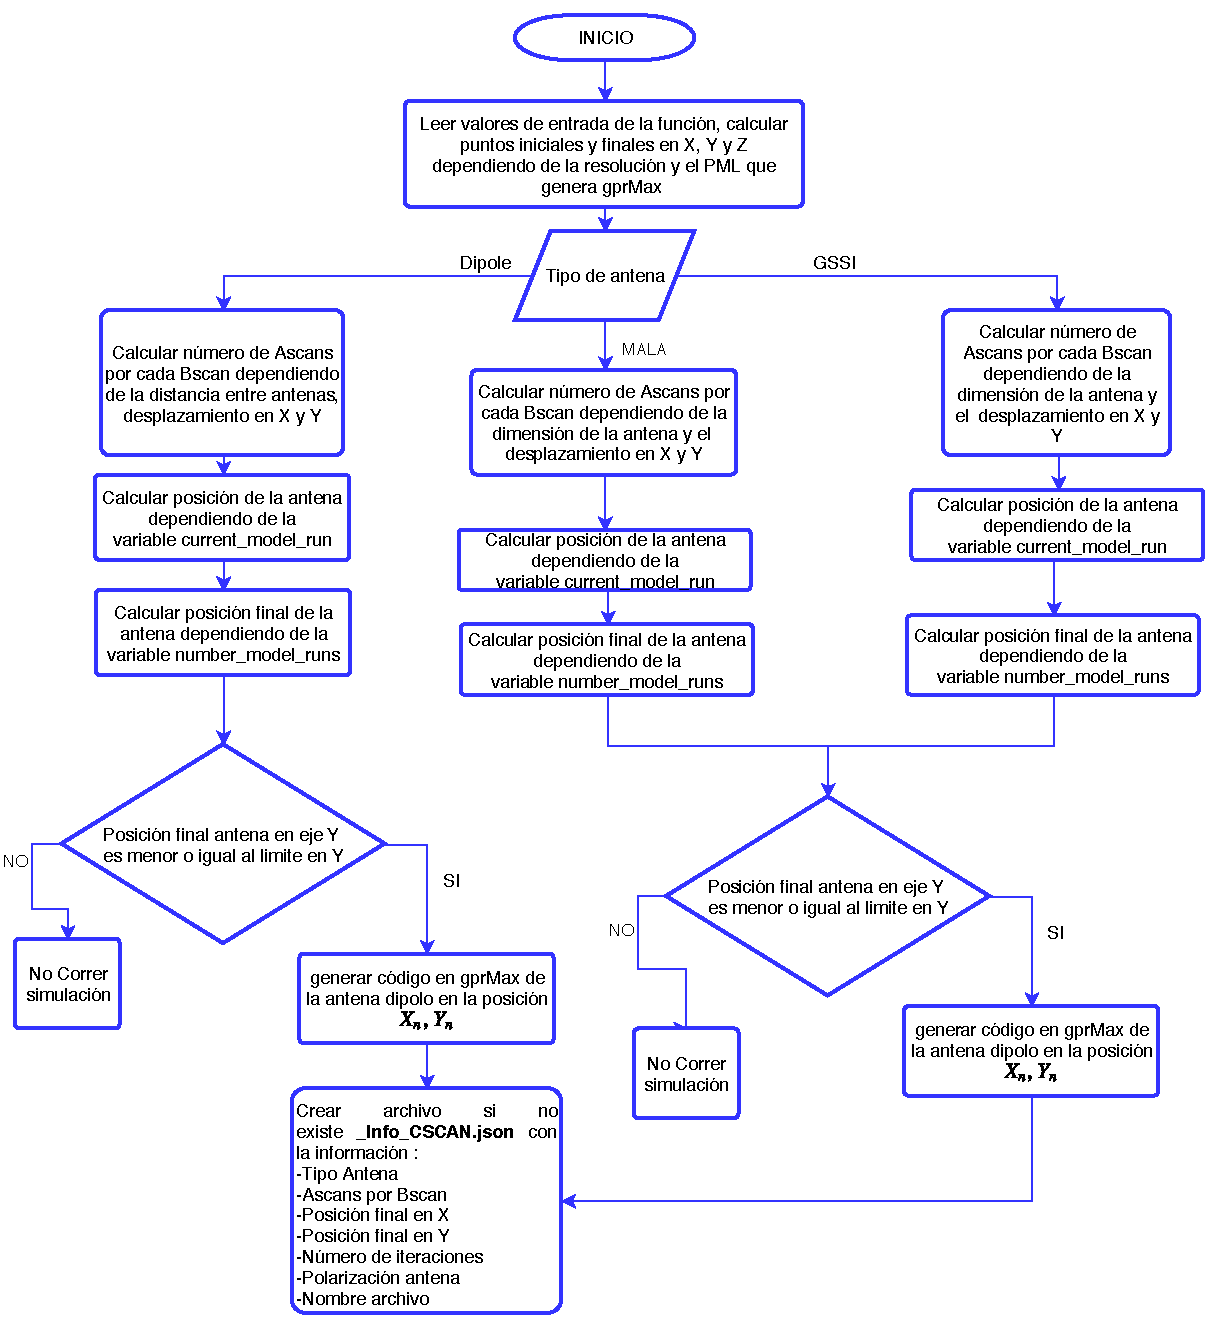
\includegraphics[height=\textheight-9cm,keepaspectratio]{chapter1/images/diagrama_flujo_cscan.pdf}
\caption{Diagrama de flujo generar trazas C}
\label{fig:FlowDiag_TrazasC}
\end{figure}
El resultado del modulo diseñado para generar trazas C en gprMax se puede puede apreciar en la  \figurename{ \ref{img:exampleCscan1GSSI}} donde se muestra los cambios de una antena GSSI realizando mediciones sobre el eje X donde se encuentra una barra metálica enterrada a  5cm de profundidad. El código implementado se encuentra en la sección de anexos como \lstlistingname{ \ref{code:generate_cscan}}. El modulo generará un archivo resultante llamado \textbf{\textit{\_Info\_CSCAN.json}} que contendrá la información del modelo simulado con el modulo implementado porque los resultados del simulador son solo trazas A. Más adelante veremos la estructura de este archivo resultante y como se utiliza para combinar las trazas A.

\begin{figure}[H]  
\centering
\subfigure[Iteración 1 en gprMax ]{
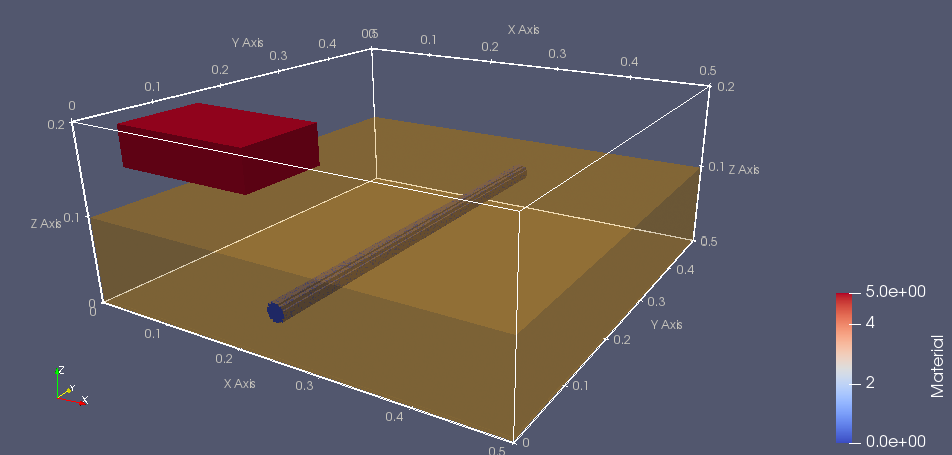
\includegraphics[width=0.3\textwidth, keepaspectratio,valign=c]{chapter1/images/sim_1_GSSI0000.png}
\label{fig:subfig1xampleCscan1GSSI}
}
\subfigure[Iteración 111 en gprMax]{
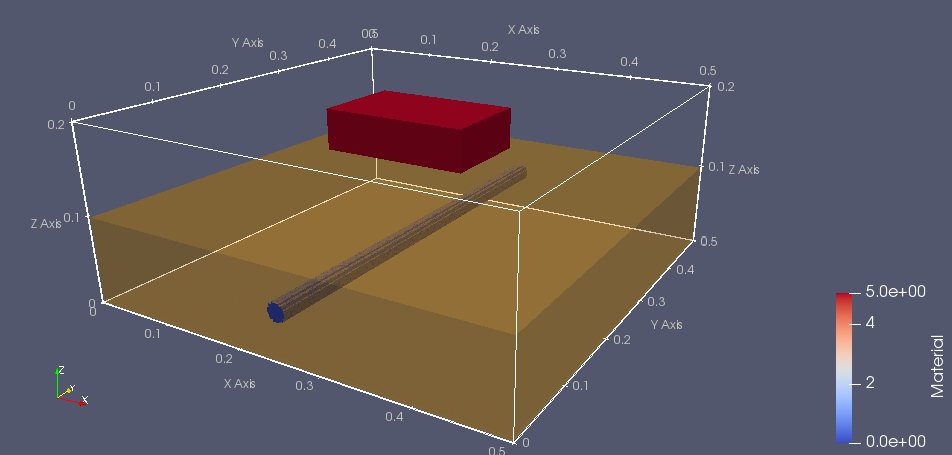
\includegraphics[width=0.3\textwidth, keepaspectratio,valign=c]{chapter1/images/sim_1_GSSI0111.png}
\label{fig:subfig2exampleCscan1GSSI}
}
\subfigure[Iteración 220 en gprMax]{
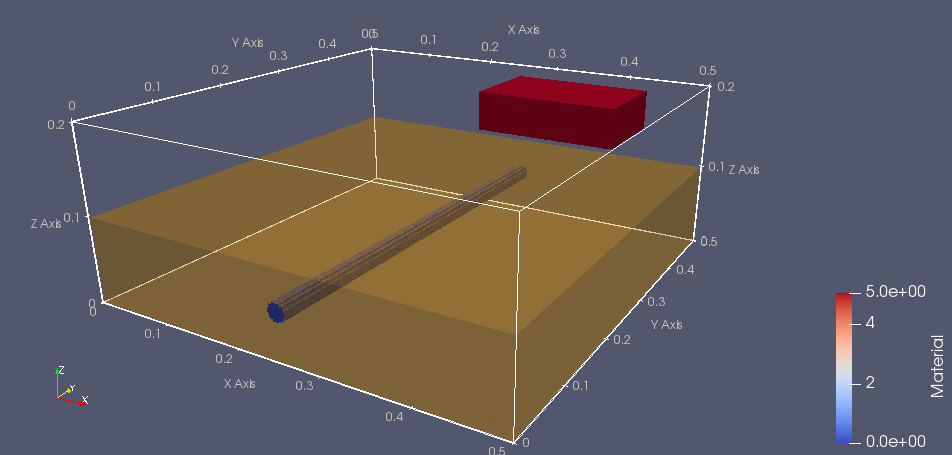
\includegraphics[width=0.3\textwidth, keepaspectratio,valign=c]{chapter1/images/sim_1_GSSI0220.png}
}

\caption{Resultado del desplazamiento de 5cm en cada eje de la antena GSSI para realizar trazas C}
\label{fig:exampleCscan1GSSI}


\end{figure}




%%%%%%%%%%%  SUBSECTION %%%%%%%%%%%%%%%%%% 
\subsection{Calculadora de iteraciones para generar Trazas C}

Para el uso correcto del módulo dentro del simulador es necesario conocer el número de iteraciones requeridas para cubrir todo el dominio en el eje \(x\) y en el eje \(y\) . Se desarrolló un programa en Python que permitiera entregar el resultado de las iteraciones según las condiciones del modelo a simular. En la \figurename{ \ref{fig:FlowDiag_calc_iter}} se encuentra el diagrama de flujo del programa y el \lstlistingname{ \ref{code:calc_iter}} el programa asociado al flujo.


\begin{figure}[H]
\centering
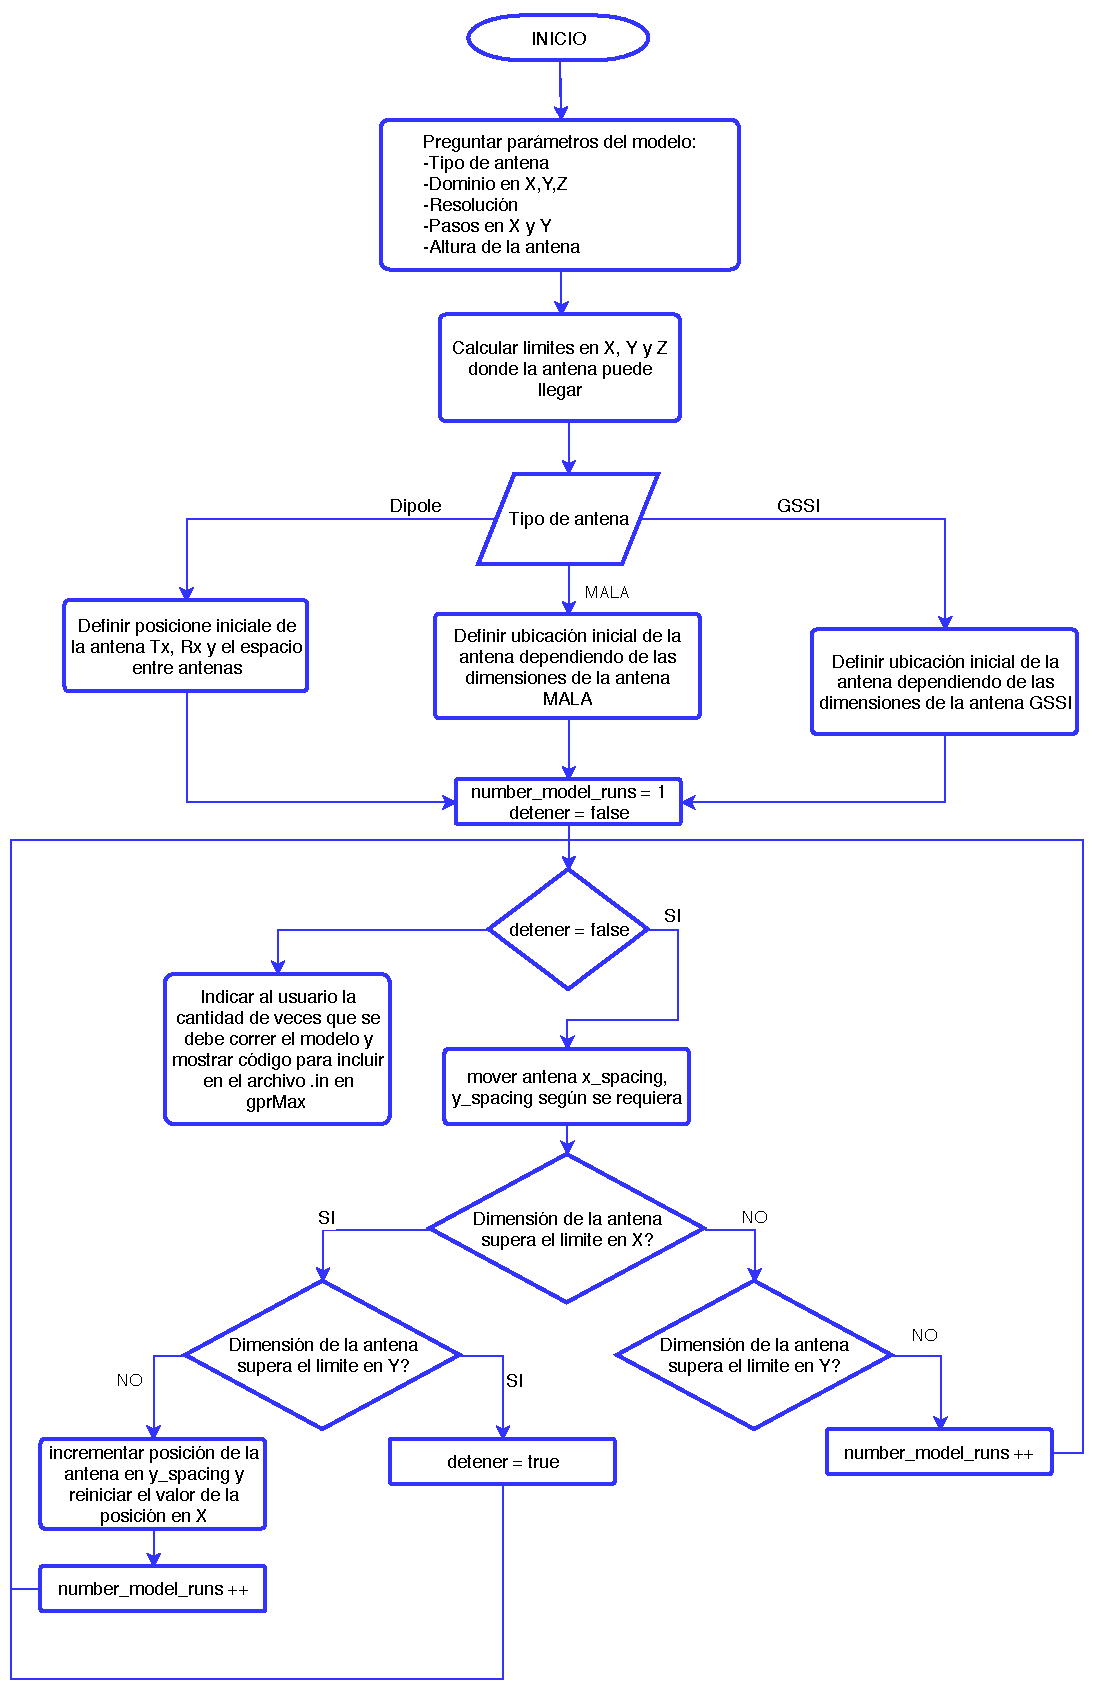
\includegraphics[height=\textheight-4.5cm,keepaspectratio]{chapter1/images/diagrama_flujo_calcular_iteraciones.pdf}
\caption{Diagrama de flujo para calcular el número de iteraciones}
\label{fig:FlowDiag_calc_iter}
\end{figure}

El programa inicia preguntando al  usuario los diferentes parámetros de simulación que van a tener en cuenta cuando se ejecute el modelo en gprMax, la \figurename{ \ref{fig:subfigParametros}} muestra las siete preguntas necesarias para encontrar el numero de iteraciones.  La  \figurename{ \ref{fig:subfigResultados}}  muestra el resultado del algoritmo indicando el numero de iteraciones a colocar en el simulador y en  \ref{fig:subfigResultadosModelo} la integración en un archivo \textbf{\textit{.in}} de gprMax


\begin{figure}[H]   
\centering
\subfigure[Indicando parámetros del modelo]{
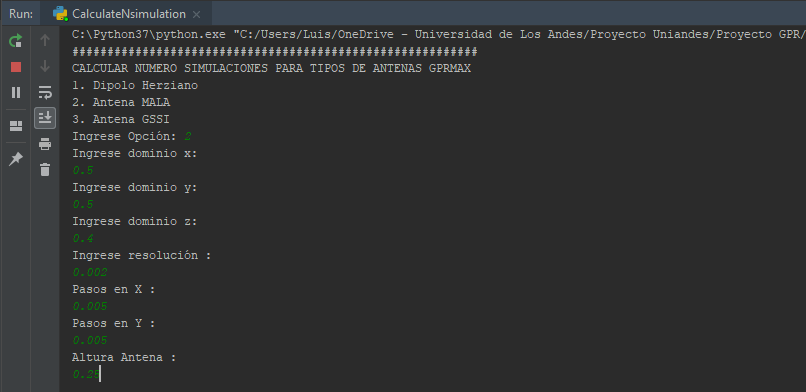
\includegraphics[width=0.7\textwidth, keepaspectratio,valign=c]{chapter1/images/iteraciones1.png}
\label{fig:subfigParametros}
}
\subfigure[Entrega de resultados del algoritmo]{
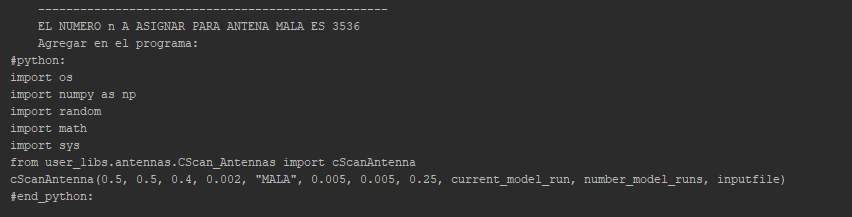
\includegraphics[width=0.7\textwidth, keepaspectratio,valign=c]{chapter1/images/iteraciones2.png}
\label{fig:subfigResultados}
}
\subfigure[Ejemplo en archivo .in gprMax]{
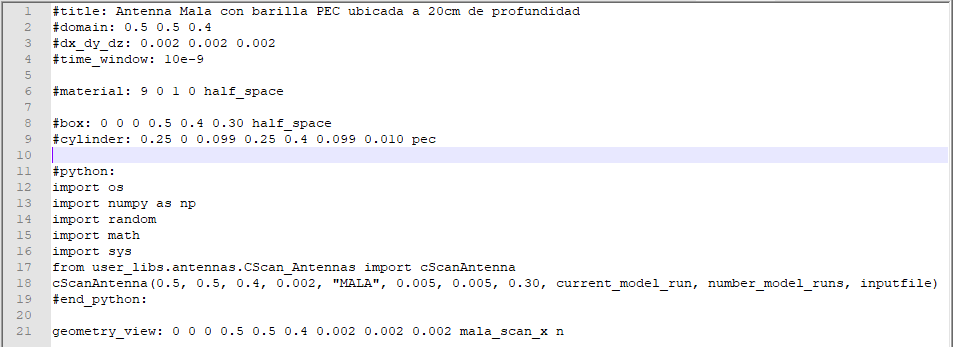
\includegraphics[width=0.7\textwidth, keepaspectratio,valign=c]{chapter1/images/ejemplo_cscan.png}
\label{fig:subfigResultadosModelo}
}

\caption{Funcionamiento algoritmo para calcular iteraciones}
\label{fig:calcularIteraciones}


\end{figure}





%%%%%%%%%%%  SUBSECTION %%%%%%%%%%%%%%%%%% 
\newpage
\subsection{Correr Múltiples Escenarios}

Para optimizar el proceso de simulación de escenarios en la herramienta gprMax, se creo un programa en Python que se encarga de leer archivos de configuración en formato \textbf{\textit{.json}} de tal forma que le permita ejecutar un número prácticamente ilimitado de modelos que contenga una carpeta, la  \figurename{ \ref{fig:flow_config_file}} muestra el diagrama de flujo utilizado en el programa para ejecutar los modelos que estén dentro de una carpeta y el \lstlistingname{ \ref{code:run_muliple}} es el algoritmo utilizado para este diagrama de flujo.

Al momento de realizar las simulaciones en gprMax debe indicarse la ruta y el nombre del archivo \textbf{\textit{.in}}, con el algoritmo desarrollado no es necesario realiza esto. Para ello se debe crear en cada carpeta de simulación un archivo llamado \textbf{\textit{configure\_model.json}}, así como se ve en la \figurename{ \ref{fig:config_file}}.  
 
\begin{figure}[H]
\centering
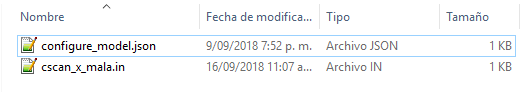
\includegraphics[width=15cm,keepaspectratio]{chapter1/images/archivos_modelo.png}
\caption{Archivo de configuración}
\label{fig:config_file}
\end{figure}

El contenido del archivo \textbf{\textit{configure\_model.json}}  debe tener la siguiente estructura 
\begin{lstlisting} []
{
    "n":2496, 
    "geometry-only":false
}
\end{lstlisting}
donde \textbf{n} corresponde al número de iteraciones que va a tener el modelo y \textbf{geometry-only} corresponde si el modelo a ejecutar solo entregará como resultado la geometría. Este ultimo parámetro es importante porque si el usuario quiere tener los archivos \textbf{\textit{.vti}} para mostrar el escenario en ParaView puede hacerlo cambiando el estado a true

\textcolor{red}{Es importante que el archivo \textbf{\textit{.in }} tenga el mismo nombre de la carpeta, de lo contrario el algoritmo no ejecutará la simulación.}

Cuando se quiera ejecutar el algoritmo es necesario tener otro archivo de configuración, este archivo contendrá las opciones el algoritmo para saber qué carpeta debe revisar y ejecutar todos los modelos que están adentro. A continuación vemos un ejemplo del archivo .json

\begin{lstlisting} []
{
"multiFolder":false,
"directory": "C:\Users\Luis\Desktop\medidas"
}
\end{lstlisting}

Si el usuario no quiere correr todos los modelos de una carpeta puede cambiar el estado de \textit{multifolder} a true, y en ella agregar la opción \textit{models}; esta opción es un arreglo que contiene el nombre de los modelos a ejecutar.

\begin{lstlisting} []
{
"multiFolder":true,
"directory": "C:\Users\Luis\Desktop\medidas",
"models" : ["cscan_x_dipole","cscan_x_gssi"]
}
\end{lstlisting}

Para ejecutar el archivo basta con colocar la siguiente linea de comando \textcolor{blue}{\textbf{python run\_file.py <url archivo .json>}}


\begin{figure}[H]
\centering
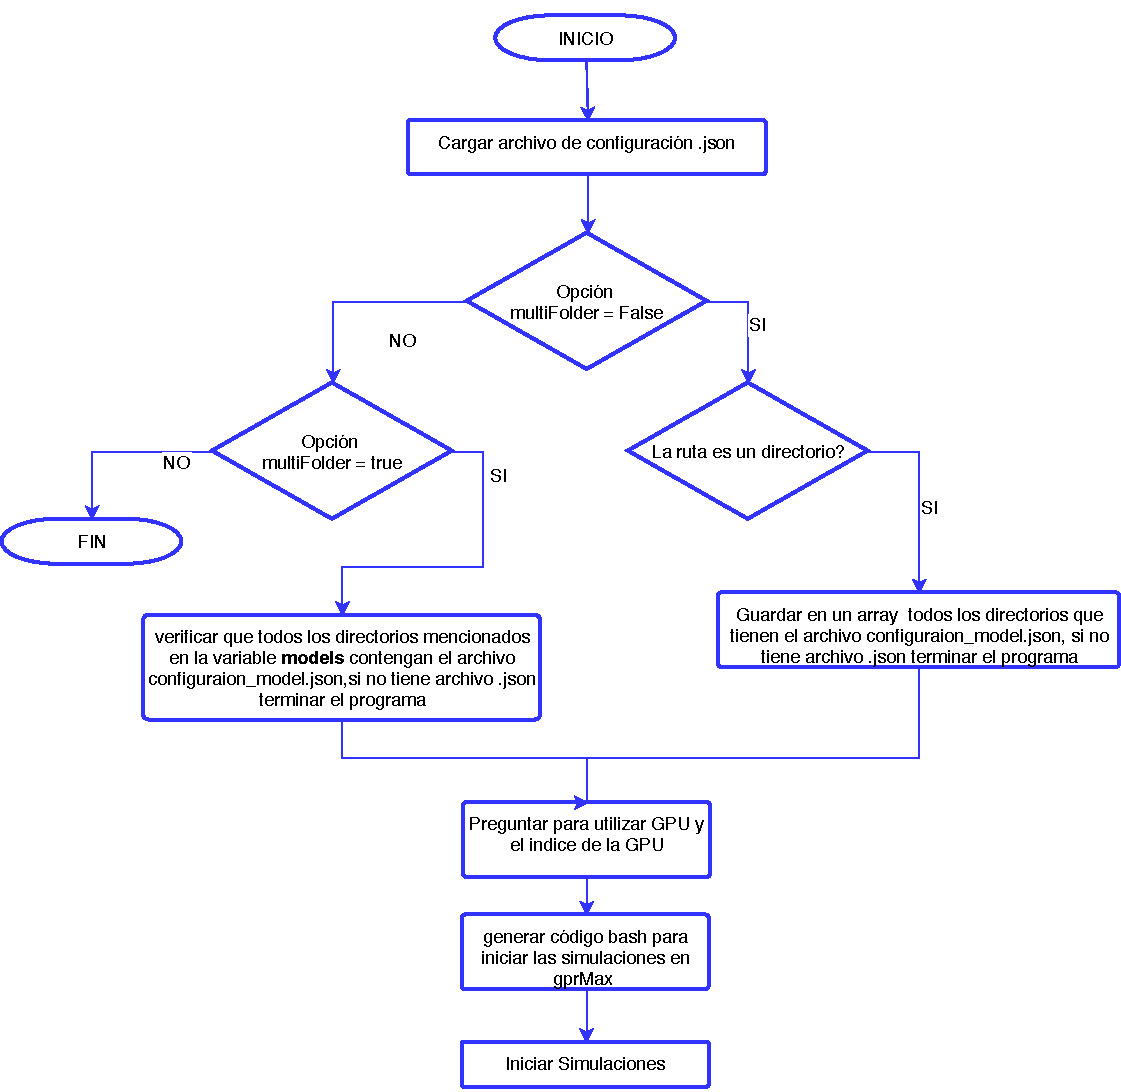
\includegraphics[height=\textheight-3.5cm,keepaspectratio]{chapter1/images/diagrama_flujo_run_multiple.pdf}
\caption{Diagrama de flujo correr múltiples escenarios}
\label{fig:flow_config_file}
\end{figure}


%%%%%%%%%%%  SUBSECTION %%%%%%%%%%%%%%%%%% 
\subsection{Combinar series de Tazas A para generar Trazas B}

Una vez gprMax termina de realizar la simulación de los modelos indicados por el usuario, en las carpetas de los diferentes modelos van a estar los archivos \textbf{\textit{.out}} que corresponden a las trazas A de las diferentes iteraciones realizadas con la librería para genera la traza C; y por otro lado va a contener un archivo de resultados llamado  \textbf{\textit{\_Info\_CSCAN.json}}, el contenido del archivo tendrá información similar a la siguiente:

\begin{lstlisting} []
{
 "antennaType": "GSSI", 
 "scansPerBScan": 52, 
 "finalPositionXEdge": 0.467, 
 "finalPositionYEdge": 0.372,
 "finalAntennaPointX": 0.375, 
 "finalAntennaPointY": 0.3175, 
 "number_model_runs": 2496, 
 "inputfile": "/home/gprmaxtest/gprMax/user_models/luis/cscan/cscan_x_gssi/cscan_x_gssi.in"
 }
\end{lstlisting}

Con esta información se modificó el archivo original \textbf{\textit{outputfiles\_merge.py}} donde deba leer el archivo  de resultados  y saber cuantas trazas A conforman una traza B. En la \figurename{ \ref{fig:merge_traces}} se observa el diagrama de flujo del programa y el \lstlistingname{  \ref{code:merge_multipleAscan}} el algoritmo desarrollado.

Para ejecutar el archivo basta con colocar la siguiente linea de comando \textcolor{blue}{\textbf{python merge\_multiple\_Ascans.py <url archivo .json>}}


Con estos códigos desarrollados en Python es posible inciar las etapas de pre-procesamiento  y migración.

\begin{figure}[H]
\centering
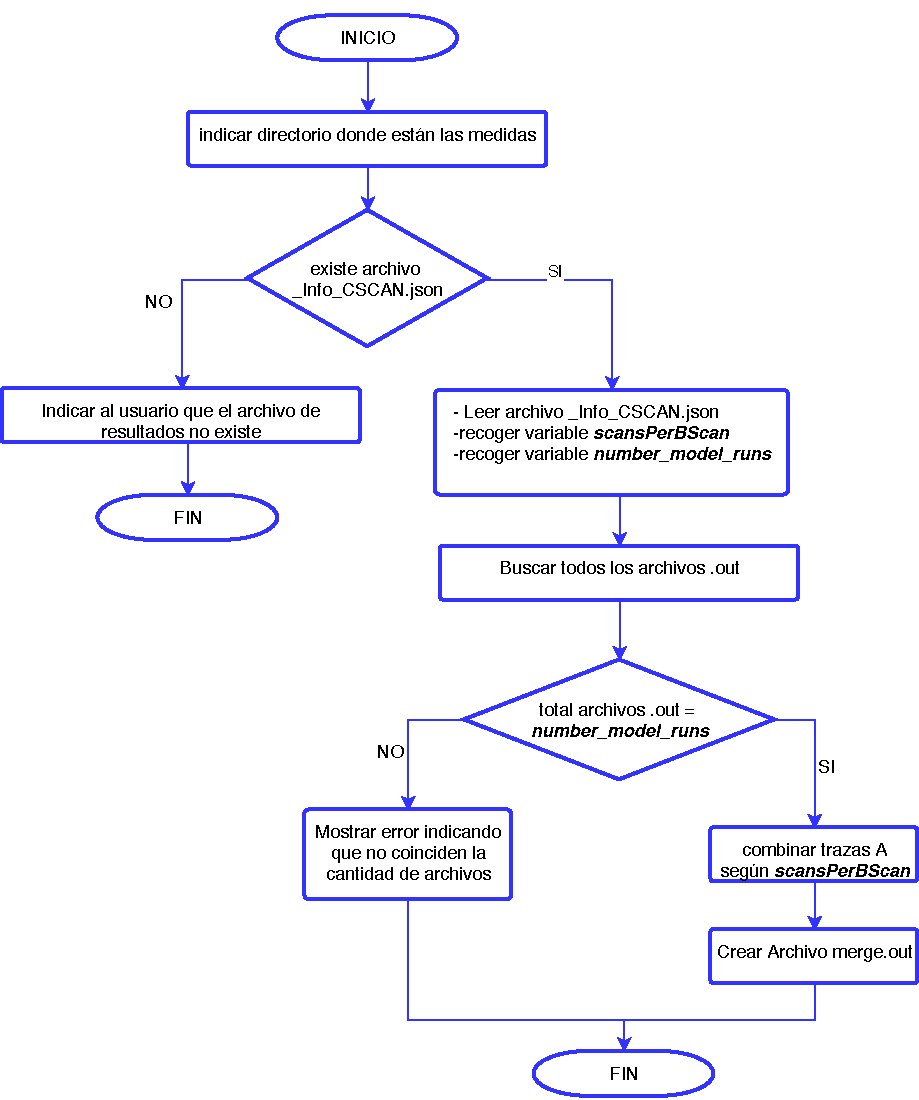
\includegraphics[height=\textheight-3.5cm,keepaspectratio]{chapter1/images/flujo_combinar_trazas.pdf}
\caption{Diagrama de flujo combinar trazas A para crear trazas B}
\label{fig:merge_traces}
\end{figure}


